\chapter{Introduction}
Named Data Networking is an interesting new paradigm in the space of network architectures. Years on since Bell Labs' work on telephony, networking research had assumed that telephony is the right model for data networking\cite{01}. This model implied that there had to be a determined route between two points for communication to happen - the setup for which was costly. This was proven not to be the case in Paul Baran's research paper titled ``On Distributed Communication Networks" in 1964, which was widely disregarded until the practical application of his work in ARPAnet(Sept,'71).MIT Senior Researcher David Clark's paper on end-to-end principle confirmed the same and it became apparent that networking solved the telephony problem. However, we are still using this same architecture which was invented as a solution for a problem that is now five decades old, and the Internet of today is not facing the same challenges. CISCO predicted in 2013\cite{02}\cite{03}, that by the end of 2017, the annual traffic of the internet would exceed 1.4 zettabytes with almost 80\% of that being video traffic.

This is why, in the age of content delivery, Named Data Networking and other Information Centric Networking architectures aim to move away from the source-destination pairwise method of IP communication which is inherently limited. Instead, NDN proposes a Name-based approach where each node in a network can request content based on the name of a piece of data it requires. 

This project aims to improve on the security implemented in Named Data Networking.


The aim of this introduction is to give background for motivation as well as lay out the structure of this paper.
\section{Motivation}
Traditional NDN: The traditional NDN architecture presents a security architecture not dissimilar to the Central Authority architecture conceptualized by Loren Kohnfelder in 1978\cite{04}. It provides a public file\cite{05} system where all nodes can check the entries for other nodes issued by a central, trusted third party called the Certificate Authority(CA) which signs each entry or `certificate'. This is all quite simple in a MiniNDN test environment, as described in the Certificates section in Chapter 2. In the case of a general or non-experimental NDN deployment\cite{06} however, this is not the case.\par 
The Network Manager would have to request a certificate verified by the CA. The manager, in turn, must also trust the CA and therefore the CA must be authentic and trusted by most networks. Trusted companies that provide this CA service include Verisign, GeoTrust,Symantec, etc... \par
The Network Manager would then provide a certificate for every node in the network which would in turn be signed by the root certificate provided by the authenticated CA. When a node wants to verify a certificate, like it would if it was receiving a Data packet, it would have to verify all of the certificates in the network hierarchy meaning it would also have to verify the root network certificate, for which it would have to contact the Certificate Authority. This means that verifying certificates can potentially involve a lot of communication.\par 
This could be avoided by introducing a Blockchain which each node could keep a copy of. This would allow nodes to verify certificates without needing to contact the CA.

To visualize this, the following example is presented in Figure 1.1. An NDN Network with an external CA has a root namespace \textbf{/ndn/} and in it there is a node called A. The root namespace is issued a certificate from the Certificate Authority which in this example is external e.g: Verisign. The root then issues a certificate for Node A. Node A in turn issues a certificate for the clock module in its namespace. These certificates allow all of the entities in the network to verify that their data is their own. If another node, like Node B for example, wants the time from Node A's clock, the node would simply express an Interest. When the clock replies with a Data packet, Node B would have to verify the data by verifying clock.cert, a.cert and root.cert. In order to verify root.cert,node B would need to contact the CA - which in the case of a real NDN environment might well be Verisign.\par
 This project recognizes that this process isn't efficient use of bandwidth as nodes would constantly have to contact the CA, performing look-ups for the sake of root certificate verification and that this can be mitigated if each node had a Blockchain of verified certificates at its disposal.
\begin{figure}[ht]
\centering
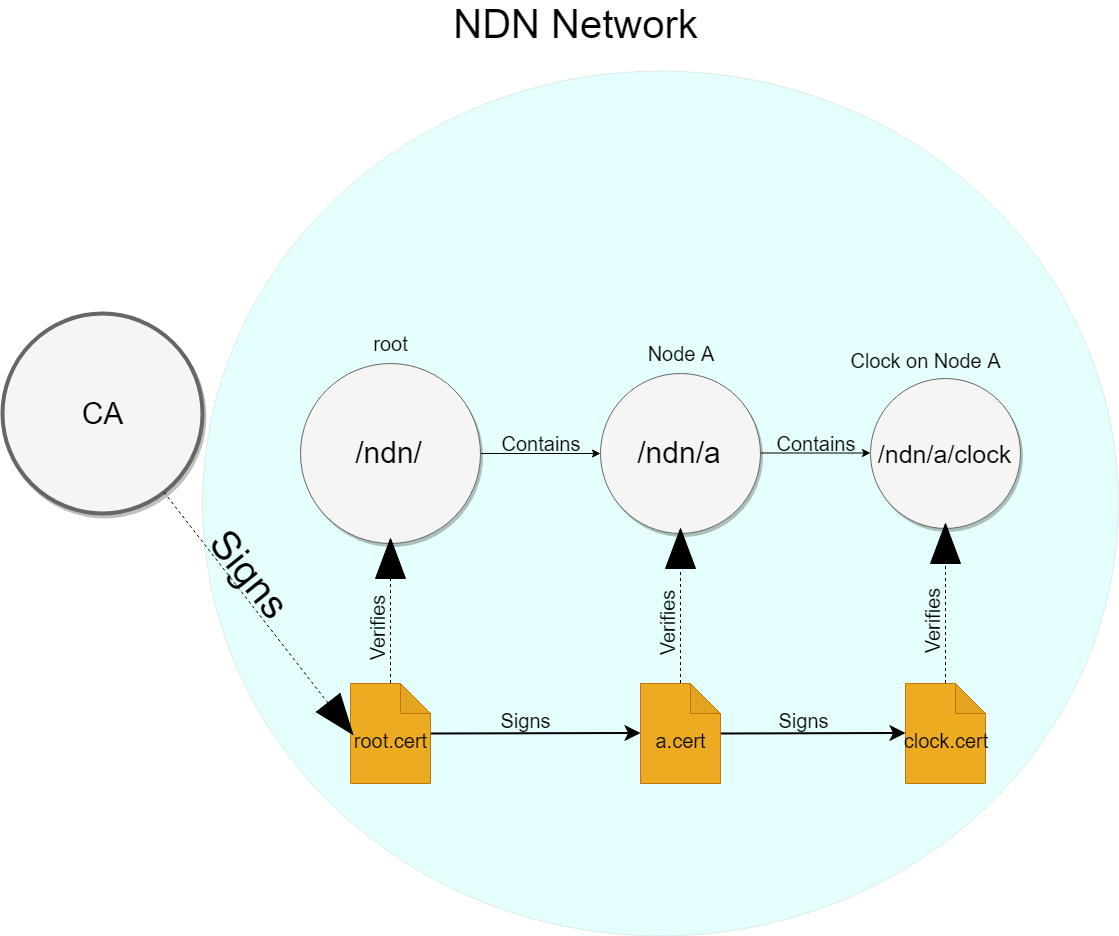
\includegraphics[width=6in,left]{certarch.png}
\caption{Certificate Hierarchy}
\end{figure}

\section{Aims}
Blockchain was an architecture proposed to store and verify transactions \textbf{reliably} in a decentralized currency system. Instead of transactions, this project aims to store certificates in a similar fashion. The goal is to do so efficiently, without increasing computational load on individual nodes in the system or increasing significantly the bandwidth use.

 It is important to note that there isn't a monetary incentive for doing this ``Proof-of-Work"\cite{07} so each network should have a dedicated group of miners which verify blocks. The assumption here is that all(or most) of the nodes will not be malicious and will not be pooling their resources to attack the network. This means that in order for one to alter the list of certificates, they would have to have more computing power than the entire network of miners. This will allow for safer communication between nodes in a network. 

\section{Road-map}
\chapquote{``Begin at the beginning," the King said gravely, ``and go on till you come to the end: then stop."}{Lewis Carroll}{Alice in Wonderland}

This paper is structured as follows: State of the Art(Lit. Review), Design and Implementation, and Evaluation.
\begin{itemize}
\item Chapter 2 contains the background information required for the scope of this project.It also contains literary reviews of the papers which discuss the State of the Art. It looks at a ranking system for the papers reviewed and also provides critique for each one. 

\item Chapter 3 discusses in detail the design of the Blockchain solution in NDN. It outlines all aspects of the conception of the data types, including solutions, design challenges and alterations that were made along the way.

\item Chapter 4 describes the implementation of this paper's solution

\item Chapter 5 goes on to evaluate the working solution by discussing different experiments and topologies. It presents graphs which illustrate the performance differences in different topologies

\end{itemize}
The paper concludes with Chapter 6 which sums up the work that's been presented and outlines any future work that might be undertaken regarding the project.